% TraceBack -- final presentation, CS455 Group 4 (7 slides)
% Build: xelatex TraceBack_Final_Presentation.tex
\documentclass[aspectratio=169,10pt]{beamer}
\usepackage{fontspec}
\usepackage{newunicodechar}
\setsansfont{Latin Modern Sans}
\setmainfont{Latin Modern Roman}
\setmonofont{Latin Modern Mono}
\newfontfamily\rupeefont{FreeSerif}[Scale=MatchUppercase]
\newunicodechar{→}{\ensuremath{\rightarrow}}
\newunicodechar{≥}{\ensuremath{\geq}}
\newunicodechar{×}{\ensuremath{\times}}
\usepackage{booktabs}
\usepackage{array}
\newcolumntype{L}[1]{>{\raggedright\arraybackslash}p{#1}}
\usepackage{tikz}
\usetikzlibrary{arrows.meta,positioning,fit,calc,backgrounds}

% ---------------- look ----------------
\definecolor{brand}{HTML}{2C41C4}
\definecolor{branddark}{HTML}{1E2E96}
\definecolor{brandwash}{HTML}{EDF0FE}
\definecolor{found}{HTML}{12694A}
\definecolor{foundwash}{HTML}{E9F5F0}
\definecolor{lost}{HTML}{B4232C}
\definecolor{lostwash}{HTML}{FBEBEC}
\definecolor{amber}{HTML}{B45309}
\definecolor{amberwash}{HTML}{FEF3C7}
\definecolor{ink}{HTML}{111827}
\definecolor{soft}{HTML}{6B7280}
\definecolor{rule}{HTML}{E5E7EB}

\setbeamertemplate{navigation symbols}{}
\setbeamercolor{normal text}{fg=ink,bg=white}
\setbeamercolor{frametitle}{fg=branddark}
\setbeamerfont{frametitle}{size=\large,series=\bfseries}
\setbeamercolor{structure}{fg=brand}
\setbeamertemplate{itemize item}{\color{brand}\textbullet}
\setbeamertemplate{itemize subitem}{\color{soft}\textendash}
\setlength{\leftmargini}{1.1em}
\setbeamertemplate{frametitle}{%
  \vspace*{0.32cm}\hspace*{-0.05cm}%
  {\usebeamerfont{frametitle}\usebeamercolor[fg]{frametitle}\insertframetitle}%
  \ifx\insertframesubtitle\empty\else\\[1pt]{\small\color{soft}\insertframesubtitle}\fi
  \par\vspace{-2pt}{\color{brand}\rule{1.2cm}{1.4pt}}\par\vspace{4pt}}
\setbeamertemplate{footline}{%
  \hspace*{0.6cm}{\tiny\color{soft}TraceBack \textperiodcentered{} IIT Kanpur Lost \& Found \textperiodcentered{} CS455 Group 4}%
  \hfill{\tiny\color{soft}\insertframenumber\,/\,7}\hspace*{0.6cm}\vspace*{0.3cm}}
\setbeamersize{text margin left=0.6cm,text margin right=0.6cm}

\newcommand{\pill}[2][brand]{{\setlength{\fboxsep}{1.6pt}\colorbox{#1!12}{\scriptsize\color{#1}\textbf{#2}}}}
\newcommand{\head}[1]{{\footnotesize\bfseries\color{branddark}#1}\par\vspace{1pt}}
\newcommand{\bignum}[2]{{\Large\bfseries\color{branddark}#1}\\[-1pt]{\scriptsize\color{soft}#2}}
\tikzset{
  b/.style={draw=brand,fill=brandwash,rounded corners=3pt,align=center,font=\scriptsize,inner sep=4pt,minimum height=0.75cm},
  g/.style={b,draw=found,fill=foundwash},
  a/.style={b,draw=amber,fill=amberwash},
  r/.style={b,draw=lost,fill=lostwash},
  ar/.style={-{Stealth[length=1.8mm]},semithick,draw=soft},
  l/.style={font=\tiny,color=soft,align=center},
}
\newcommand{\tblogo}[1][0.03]{%
\begin{tikzpicture}[scale=#1]
  \shade[left color=brand!80,right color=branddark,rounded corners=8pt] (0,0) rectangle (64,64);
  \draw[white,opacity=0.75,line width=1pt,line cap=round,dash pattern=on 0.1pt off 5pt]
     (12,12) .. controls (14,24) and (30,18) .. (30,28) .. controls (30,36) and (22,38) .. (30,42);
  \fill[found!40] (12,12) circle (3.4);
  \fill[white] (42,20) .. controls (42,20) and (28,32.4) .. (28,42.3)
     .. controls (28,49.9) and (34.3,56) .. (42,56) .. controls (49.7,56) and (56,49.9) .. (56,42.3)
     .. controls (56,32.4) and (42,20) .. (42,20) -- cycle;
  \fill[brand] (42,42.5) circle (5.2);
\end{tikzpicture}}

\begin{document}

% ================= 1. Title and team =================
{\setbeamertemplate{footline}{}
\begin{frame}
\begin{columns}[c,onlytextwidth]
\begin{column}{0.38\textwidth}
\tblogo[0.026]\\[0.3cm]
{\fontsize{26}{28}\selectfont\bfseries\color{branddark}TraceBack}\\[0.08cm]
{\small\color{soft}IIT Kanpur Lost \& Found Portal}\\[0.4cm]
{\footnotesize Report it. Hand it in.\\ Get it back, to the right person.}\\[0.55cm]
{\tiny\color{soft}
CS455 Software Engineering \textperiodcentered{} 2026-27\\
Group 4 \textperiodcentered{} Prof.\ Priyanka Bagade\\[3pt]
Live: \texttt{16-176-186-149.sslip.io}\\
Code: \texttt{github.com/cs455project/campus-lost-and-found}}
\end{column}
\begin{column}{0.58\textwidth}
\head{Team and responsibilities}
\scriptsize
\renewcommand{\arraystretch}{1.45}
\begin{tabular}{@{}L{2.55cm}L{4.95cm}@{}}
\toprule
\textbf{Ankit Agarwal} & Foundation, OTP sign-in, roles, profiles, listings \\
\textbf{Bhanu Pratap} & Lost and found reports, photos, search \\
\textbf{Ankit Kumar Dubey} & Claims, approval rules, handover \\
\textbf{Dev Sachan} & Guard custody, item page, app shell \\
\textbf{Soumyaranjan Sahu} & Admin, jobs, email, audit; D3 testing, AWS deploy \\
\textbf{Rohit Yadav} & Agentic AI: matching agent and chat assistant \\
\bottomrule
\end{tabular}
\end{column}
\end{columns}
\end{frame}}

% ================= 2. Problem, objectives, roles, features =================
\begin{frame}[t]{The problem and what we set out to do}
\begin{columns}[T,onlytextwidth]
\begin{column}{0.46\textwidth}
\head{Problem}
\scriptsize
Lost items on campus are chased through WhatsApp groups and notice boards. Found items sit in hostels and offices where no one can search them, and they often go to whoever asks first, with no proof of ownership.
\vspace{6pt}

\head{Objectives}
\begin{itemize}\setlength{\itemsep}{0pt}\scriptsize
\item One place to report and search lost and found items
\item A verified chain of custody at SIS security offices
\item Handover only after a real ownership check
\item AI that suggests matches but never decides
\item Privacy by design, within free-tier cost
\end{itemize}
\end{column}
\begin{column}{0.50\textwidth}
\head{User roles}
\scriptsize
\renewcommand{\arraystretch}{1.15}
\begin{tabular}{@{}l L{3.9cm}@{}}
\pill{Student} & report, search, claim with private proof \\
\pill[found]{SIS Guard} & receive, hold, review claims, hand over \\
\pill[amber]{Admin} & manage guards and admins, read audit logs \\
\end{tabular}
\vspace{5pt}

\head{Key features}
\begin{itemize}\setlength{\itemsep}{0pt}\scriptsize
\item Reports with photos; search with filters
\item AI matches with reasons; the owner is emailed
\item \textbf{Ask TraceBack}: a chat assistant for students
\item Found ID card \textrightarrow{} owner emailed (on-server OCR)
\item Custody history: who held it, where, when
\item Claims with private proof, guard review, ID-checked handover
\end{itemize}
\end{column}
\end{columns}
\end{frame}

% ================= 3. Requirements and their evolution =================
\begin{frame}[t]{Requirements engineering and how they evolved}
\begin{columns}[T,onlytextwidth]
\begin{column}{0.37\textwidth}
\head{How we captured them}
\begin{itemize}\setlength{\itemsep}{1pt}\scriptsize
\item Stakeholders: students, SIS guards, admin; use cases and a literature review (D1)
\item \textbf{28 user stories} in Jira, SCRUM-10 to 57, with acceptance criteria
\item 11 functional groups (AUTH, REP, SRCH, CUS, CLM, CON, AI, ADM \dots)
\item Non-functional: security, privacy, concurrency, performance, reliability, AI cost
\item Agent behaviour as requirements: autonomous, bounded, human-only, prohibited
\end{itemize}
\vspace{6pt}

\begin{tikzpicture}
\fill[found] (0,0) rectangle (3.6,0.2); \fill[amber] (3.6,0) rectangle (4.1,0.2); \fill[lost!70] (4.1,0) rectangle (4.6,0.2);
\node[anchor=south west,font=\tiny,color=found,inner sep=1pt] at (0,0.22) {\textbf{22 of 28 stories delivered}};
\node[anchor=north east,font=\tiny,color=soft,inner sep=1pt] at (4.6,-0.02) {3 dropped, 3 descoped};
\end{tikzpicture}
\end{column}
\begin{column}{0.59\textwidth}
\head{19 recorded changes; the ones that mattered most}
\scriptsize
\renewcommand{\arraystretch}{1.28}
\begin{tabular}{@{}L{3.5cm}L{4.2cm}@{}}
\toprule
\textbf{Change} & \textbf{Reason} \\
\midrule
Every handover goes through a guard; direct finder handover dropped & With no third party, anyone could claim a phone \\
Item chat dropped & It leaks the details used to verify ownership \\
ID-card owner alert by local OCR added & IDs returned fast, photo never shared \\
AI called only when unsure, 500 calls a day & Stay inside free tiers \\
Verification score, visit slots descoped (D3) & Guard review + ID check already verify; time went to testing \\
\bottomrule
\end{tabular}
\end{column}
\end{columns}
\end{frame}

% ================= 4. Architecture =================
\begin{frame}[t]{System architecture and design patterns}
\begin{columns}[T,onlytextwidth]
\begin{column}{0.58\textwidth}
\centering
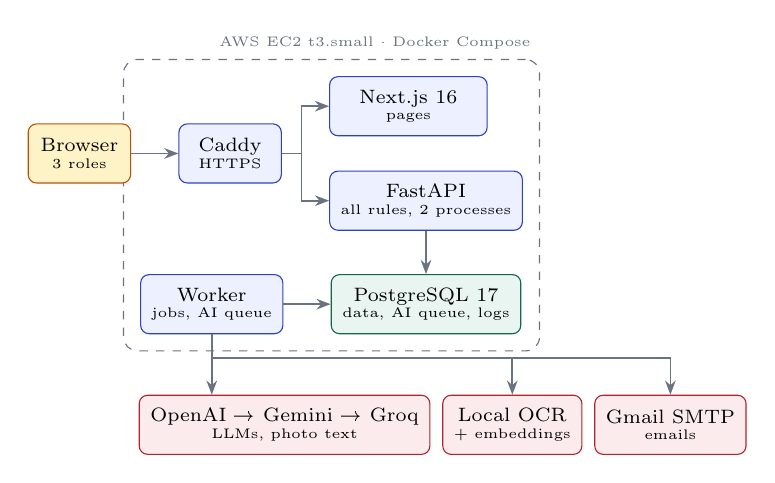
\begin{tikzpicture}[node distance=0.5cm]
\node[a,minimum width=1.3cm] (u) {Browser\\[-2pt]\tiny 3 roles};
\node[b,right=0.6cm of u,minimum width=1.3cm] (c) {Caddy\\[-2pt]\tiny HTTPS};
\node[b,right=0.6cm of c,yshift=0.6cm,minimum width=2.0cm] (f) {Next.js 16\\[-2pt]\tiny pages};
\node[b,right=0.6cm of c,yshift=-0.6cm,minimum width=2.0cm] (api) {FastAPI\\[-2pt]\tiny all rules, 2 processes};
\node[g,below=0.55cm of api,minimum width=2.0cm] (db) {PostgreSQL 17\\[-2pt]\tiny data, AI queue, logs};
\node[b,left=0.6cm of db,minimum width=1.6cm] (w) {Worker\\[-2pt]\tiny jobs, AI queue};
\draw[ar] (u) -- (c);
\draw[ar] (c.east) -- ++(0.25,0) |- (f.west);
\draw[ar] (c.east) -- ++(0.25,0) |- (api.west);
\draw[ar] (api) -- (db);
\draw[ar] (w) -- (db);
\begin{scope}[on background layer]
\node[draw=soft,dashed,rounded corners=5pt,fit=(c)(f)(api)(db)(w),inner sep=6pt] (z) {};
\end{scope}
\node[font=\tiny,color=soft,anchor=south east] at (z.north east) {AWS EC2 t3.small \textperiodcentered{} Docker Compose};
\node[r,below=0.55cm of z.south west,anchor=north west,minimum width=1.6cm,xshift=0.2cm] (llm) {OpenAI \textrightarrow{} Gemini \textrightarrow{} Groq\\[-2pt]\tiny LLMs, photo text};
\node[r,right=0.15cm of llm,minimum width=1.5cm] (ocr) {Local OCR\\[-2pt]\tiny + embeddings};
\node[r,right=0.15cm of ocr,minimum width=1.3cm] (mail) {Gmail SMTP\\[-2pt]\tiny emails};
\draw[ar] (w.south) -- (w.south |- llm.north) ;
\draw[ar] (w.south) ++(0,-0.3) -| (ocr.north);
\draw[ar] (w.south) ++(0,-0.3) -| (mail.north);
\end{tikzpicture}
\end{column}
\begin{column}{0.39\textwidth}
\head{How the parts interact}
\begin{itemize}\setlength{\itemsep}{0pt}\scriptsize
\item Only Caddy is public: it serves the pages and forwards \texttt{/api} to FastAPI; the API and database have no public port
\item The API owns every rule and only \emph{queues} slow work
\item The worker calls AI and email, so no page waits on them
\end{itemize}
\vspace{4pt}
\head{Design patterns}
\begin{itemize}\setlength{\itemsep}{0pt}\scriptsize
\item \textbf{Layers:} routers \textrightarrow{} services \textrightarrow{} models
\item \textbf{State machines} for item and claim status
\item \textbf{Producer--consumer queue} with \texttt{SKIP LOCKED}
\item \textbf{Strategy:} rule-based or agent matcher
\item \textbf{Fallback chain:} OpenAI \textrightarrow{} Gemini \textrightarrow{} Groq \textrightarrow{} rules
\item \textbf{Append-only event logs} for custody and claims
\end{itemize}
\end{column}
\end{columns}
\end{frame}

% ================= 5. Decisions, workflow, traceability =================
\begin{frame}[t]{Engineering decisions, workflow and traceability}
\begin{columns}[T,onlytextwidth]
\begin{column}{0.42\textwidth}
\head{Decisions that shaped the system}
\scriptsize
\renewcommand{\arraystretch}{1.3}
\begin{tabular}{@{}L{1.55cm}L{4.1cm}@{}}
\toprule
\textbf{Double allocation} & Row locks (item, then claim) \emph{plus} a partial unique index \\
\textbf{Sign-in} & One-time email code, stored hashed; server-side session in an HttpOnly cookie, not a JWT \\
\textbf{AI} & The model proposes; code checks ids, dates, thresholds \\
\textbf{Privacy} & ID-card photos never leave our server \\
\textbf{Hosting} & One EC2 with Compose, not Kubernetes: fits the load and the budget \\
\bottomrule
\end{tabular}
\end{column}
\begin{column}{0.54\textwidth}
\head{Jira \textrightarrow{} GitHub workflow}
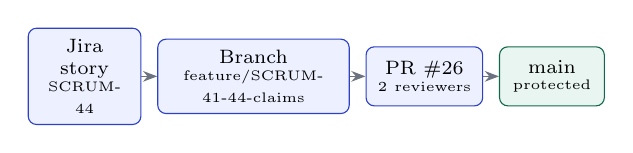
\begin{tikzpicture}[node distance=0.2cm, every node/.append style={minimum height=0.62cm,inner sep=2.5pt}]
\node[b,text width=1.15cm] (j) {Jira story\\[-2pt]\tiny SCRUM-44};
\node[b,right=of j,text width=2.15cm] (br) {Branch\\[-2pt]\tiny feature/SCRUM-41-44-claims};
\node[b,right=of br,text width=1.2cm] (pr) {PR \#26\\[-2pt]\tiny 2 reviewers};
\node[g,right=of pr,text width=1.05cm] (m) {main\\[-2pt]\tiny protected};
\draw[ar] (j)--(br); \draw[ar] (br)--(pr); \draw[ar] (pr)--(m);
\end{tikzpicture}\\[2pt]
{\scriptsize 18 story PRs (\#11 to \#28), the key in every branch, commit and PR \textperiodcentered{} 36 reviews, 6 per member \textperiodcentered{} CODEOWNERS and branch protection \textperiodcentered{} D3 fixes on \texttt{d3/integration}\par}
\vspace{6pt}

\head{One requirement, traced end to end}
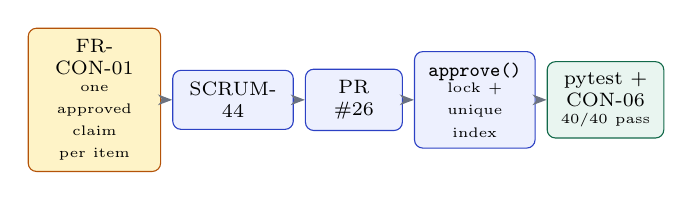
\begin{tikzpicture}[node distance=0.14cm, every node/.append style={minimum height=0.72cm,inner sep=2.5pt}]
\node[a,text width=1.4cm] (r) {FR-CON-01\\[-2pt]\tiny one approved claim per item};
\node[b,right=of r,text width=1.25cm] (s) {SCRUM-44};
\node[b,right=of s,text width=0.95cm] (p) {PR \#26};
\node[b,right=of p,text width=1.25cm] (c) {\texttt{approve()}\\[-2pt]\tiny lock + unique index};
\node[g,right=of c,text width=1.2cm] (t) {pytest + CON-06\\[-2pt]\tiny 40/40 pass};
\draw[ar] (r)--(s); \draw[ar] (s)--(p); \draw[ar] (p)--(c); \draw[ar] (c)--(t);
\end{tikzpicture}
\end{column}
\end{columns}
\end{frame}

% ================= 6. Agentic AI =================
\begin{frame}[t]{Agentic AI: two agents, one brain, firm guardrails}
\centering
\begin{tikzpicture}[x=1cm,y=1cm,
  st/.style={b,minimum height=0.85cm,anchor=west},
  lane/.style={anchor=west,align=left,text width=2.25cm,font=\scriptsize}]
% ---- lane 1: matching agent ----
\node[lane] at (0,2.2) {\textbf{\color{branddark}Matching agent}\\[-1pt]{\tiny\color{soft}runs by itself on every new report}};
\node[a,st,text width=1.5cm] (n)  at (2.5,2.2)  {New report\\[-2pt]\tiny lost or found};
\node[st,text width=1.95cm] (v)  at (4.6,2.2) {Reads the photo\\[-2pt]\tiny brand, colour, marks};
\node[st,text width=1.95cm] (sh) at (7.15,2.2) {Shortlist\\[-2pt]\tiny embeddings + rules};
\node[st,text width=2.2cm,line width=0.9pt] (ag) at (9.7,2.2) {\textbf{Agent reasons}\\[-2pt]\tiny search, compare, explain};
\node[g,st,text width=1.75cm] (o)  at (12.4,2.2) {Owner emailed\\[-2pt]\tiny match + the reason};
\draw[ar] (n)--(v); \draw[ar] (v)--(sh); \draw[ar] (sh)--(ag); \draw[ar] (ag)--(o);
\draw[ar,dashed] (sh.north) -- ++(0,0.3) -| node[l,pos=0.27,above,inner sep=1pt]{obvious match: no LLM call, no cost} (o.north);
% ---- the shared brain ----
\node[anchor=west,fill=branddark,text=white,rounded corners=3pt,minimum height=0.6cm,minimum width=11.95cm,font=\scriptsize] (brain) at (2.5,1.0)
  {\textbf{One LLM chain}\quad OpenAI \textrightarrow{} Gemini \textrightarrow{} Groq \quad{\tiny\color{white!75!brand}if one fails the next answers; if all fail, matching falls back to rules}};
\draw[{Stealth[length=1.6mm]}-{Stealth[length=1.6mm]},semithick,draw=branddark] (ag.south) -- (ag.south |- brain.north);
% ---- lane 2: chat assistant ----
\node[lane] at (0,-0.2) {\textbf{\color{branddark}Ask TraceBack}\\[-1pt]{\tiny\color{soft}chat assistant, answers students}};
\node[a,st,text width=1.95cm] (q) at (2.5,-0.2) {Student asks\\[-2pt]\tiny ``anyone found a black wallet?''};
\node[st,text width=2.2cm,line width=0.9pt] (tool) at (9.7,-0.2) {\textbf{Agent uses tools}\\[-2pt]\tiny found items, my claims, offices};
\node[g,st,text width=1.75cm] (ans) at (12.4,-0.2) {Answer + links\\[-2pt]\tiny FND-0012 opens the item};
\draw[ar] (q) -- node[l,above,inner sep=1pt]{question + recent chat} (tool);
\draw[ar] (tool)--(ans);
\draw[{Stealth[length=1.6mm]}-{Stealth[length=1.6mm]},semithick,draw=branddark] (tool.north) -- (tool.north |- brain.south);
% ---- guardrails ----
\node[anchor=west,font=\footnotesize\bfseries,color=branddark] at (0,-1.3) {Guardrails: the AI suggests, people decide};
\tikzset{gr/.style={draw,rounded corners=3pt,anchor=north west,text width=3.2cm,minimum height=1.05cm,align=left,font=\tiny,inner sep=3.5pt}}
\node[gr,draw=found,fill=foundwash]  at (0,-1.6)    {{\scriptsize\bfseries\color{found}Does on its own}\\ rank matches, widen a search, explain why, answer questions};
\node[gr,draw=amber,fill=amberwash]  at (3.62,-1.6) {{\scriptsize\bfseries\color{amber}Only within limits}\\ email an owner: score ≥ 0.7, item held at an office, only once};
\node[gr,draw=brand,fill=brandwash]  at (7.24,-1.6) {{\scriptsize\bfseries\color{brand}Only a guard}\\ approve or reject a claim, hand over, move custody};
\node[gr,draw=lost,fill=lostwash]    at (10.86,-1.6){{\scriptsize\bfseries\color{lost}Never}\\ see names, emails, phone or roll numbers; run SQL; change a status};
\node[anchor=north west,font=\tiny,color=soft,text width=14.4cm,align=left] at (0,-2.78)
  {Read-only tools \textperiodcentered{} code checks every id and date the model returns \textperiodcentered{} found ID cards are read only on our server \textperiodcentered{} daily and per-student limits \textperiodcentered{} every run logged, no chat text stored};
\end{tikzpicture}
\end{frame}

% ================= 7. Testing ... lessons =================
\newcommand{\stat}[2]{\begin{minipage}[t]{2.2cm}\raggedright{\Large\bfseries\color{branddark}#1}\par\vspace{1pt}{\scriptsize\color{soft}#2\par}\end{minipage}}
\begin{frame}[t]{Testing, debugging, security, performance and deployment}
\begin{columns}[T,onlytextwidth]
\begin{column}{0.60\textwidth}
\stat{479}{unit + integration tests}\hfill\stat{97.8\%}{of lines, 91.2\% of branches}\hfill\stat{15/15}{browser system tests}\\[8pt]
\stat{23/23}{attacks stopped; 2 audits clean}\hfill\stat{14 × 40}{concurrency races, all pass}\hfill\stat{10/10}{failures recover by themselves}
\vspace{8pt}

\head{Debugging: 25 defects found, all 25 fixed}
\scriptsize
\textbf{Worst (critical):} the API locked up at 25 users. A profiler showed 40 threads waiting on 15 database connections. We capped requests in flight and sized the pool. \textbf{Now:} 100 users, 0 errors, about 250 requests/s (was 71); 0.8\,MB per page (was 18\,MB).\\[3pt]
\textbf{Others:} double handover in a race (row locks); GPS left in photos (stripped); crashed AI jobs lost (re-queued); bare 500 when the database was down (clear 503).
\end{column}
\begin{column}{0.36\textwidth}
\head{Security}
{\scriptsize STRIDE model of 22 threats, each with a control in the code. What remains is operational: key rotation and MFA.\par}
\vspace{5pt}

\head{Deployment}
{\scriptsize AWS EC2 t3.small (Sydney), 5 Docker containers, Caddy auto-HTTPS, one-command deploy; about US\$25 a month, paid by free credits.\par}
\vspace{5pt}

\head{Lessons}
\begin{itemize}\setlength{\itemsep}{0pt}\scriptsize
\item Test concurrency and load from sprint one: they found our worst bugs
\item Measure, don't assume: the bottleneck wasn't where we guessed
\item Leaving data out beats inventing it
\end{itemize}
\end{column}
\end{columns}
\end{frame}

\end{document}
